\exercise{Enhancement}
\subsection*{a - \texttt{IPlogenhance}}
Sometimes it can be desirable to increase the intensity of low-intensity pixels without affecting high-intensity pixels too much. A way to achieve this goal is by compressing the dynamic range of an image. By applying the log transform, an image may become more insightful than when the dynamic range is too large. The log transformation is: 
\[
  s = c\mbox{ }log(1+r)
\]
In this formula the value $r$ represents the value of the pixel the transformation is applied to. The value $c$ is a parameter chosen by the user. Implementing this formula is fairly straightforward in \textit{MATLAB} and we arrived at this solution directly by implementing the formula. The following \textit{MATLAB} code applies the log transformation to an image. 
\matlabexternal{IPlogenhance.m}
Here the type of \verb image  is a $y \times x$-matrix. The output image is a $y \times x$-matrix with the transformation applied.

\subsection*{b - Enhancing a fractured spine}
In order to make sure the implementation is correct and the log transformation is useful, the operation is applied to an image that could benefit from a compressed dynamic range.

Figures~\ref{fig:withoutEnhancement} to~\ref{fig:withMoreEnhancement} are pictures of a fractured spine, but Figure~\ref{fig:withEnhancement} has the log transformation applied to it with $c = 1.75$ and Figure~\ref{fig:withMoreEnhancement} has the log transformation with $c=3$. 
We have chosen two values for the transformation, since the higher value (Figure \ref{fig:withMoreEnhancement}) shows more detail in the darker areas, whereas there is still some detail in the lighter areas for the lower value of $c$ in Figure \ref{fig:withEnhancement}. We have chosen these values specifically because we felt it has the best trade-off in enhancing areas that were less visible while not overexposing values that already had a high intensity.

\begin{figure}[!Htb]
 \centering
 \begin{subfigure}[b]{0.32\linewidth}
  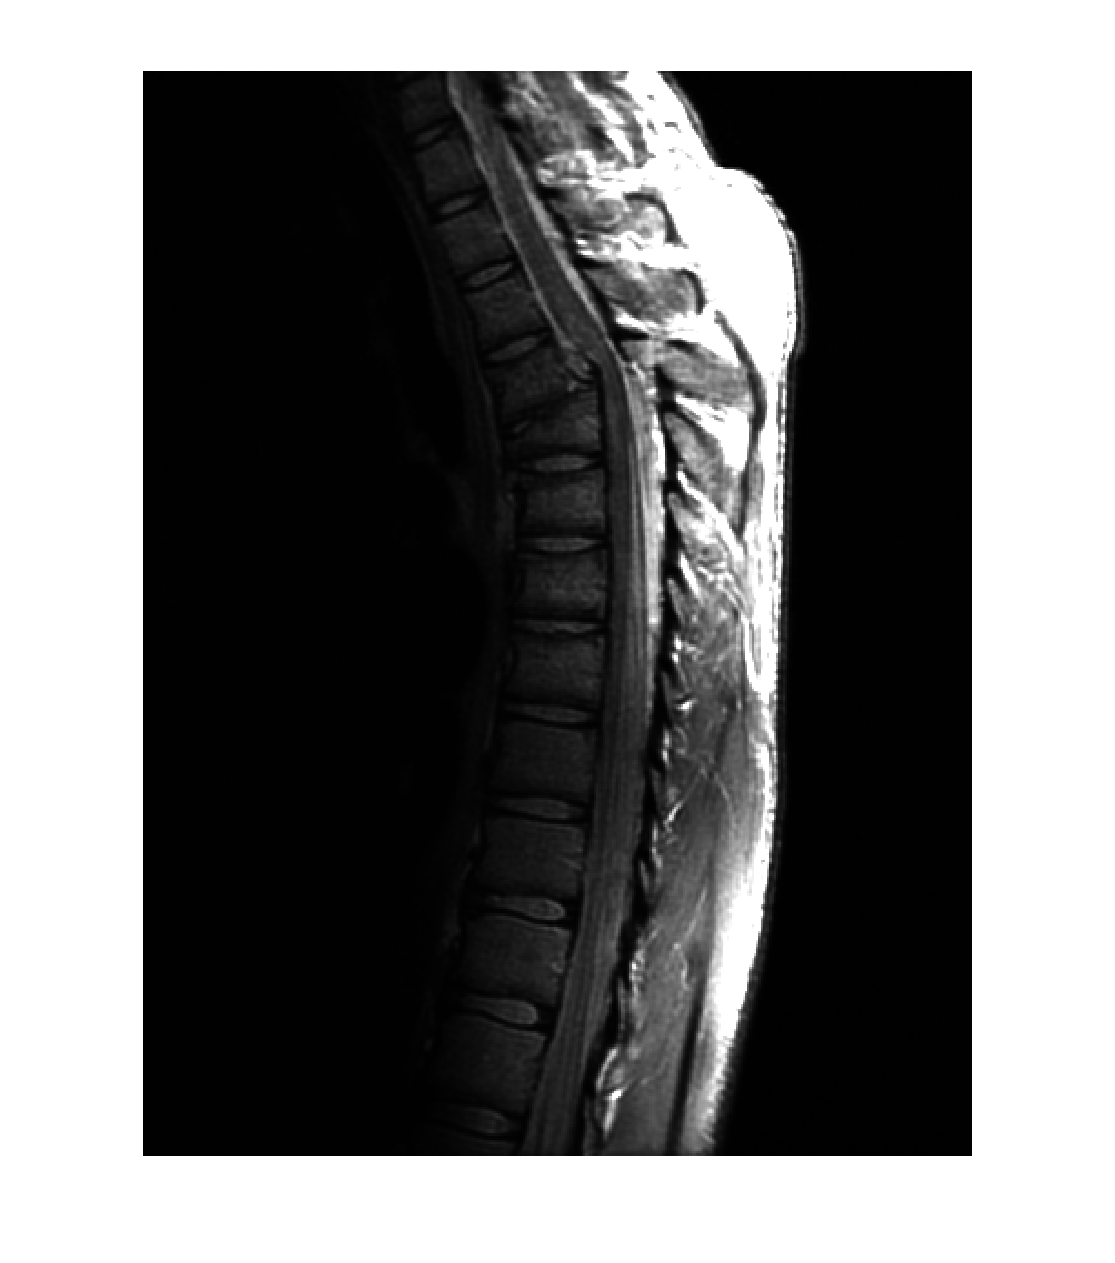
\includegraphics[width=\textwidth]{breukLelijk.eps} 
  \caption{No enhancement}
  \label{fig:withoutEnhancement} 
 \end{subfigure}
 \begin{subfigure}[b]{0.32\linewidth}
  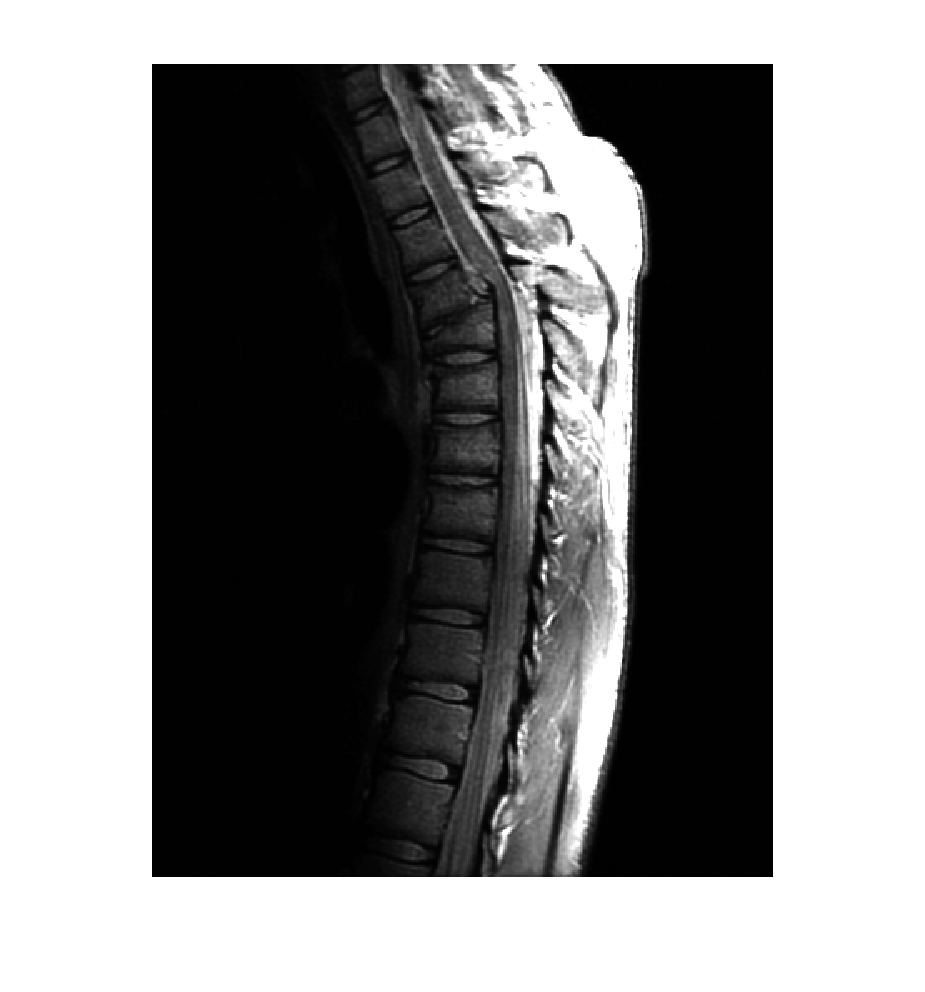
\includegraphics[width=\textwidth]{breukMooi.eps}
  \caption{Enhanced with \(c=1.75\)}
  \label{fig:withEnhancement}
 \end{subfigure}
\begin{subfigure}[b]{0.32\linewidth}
  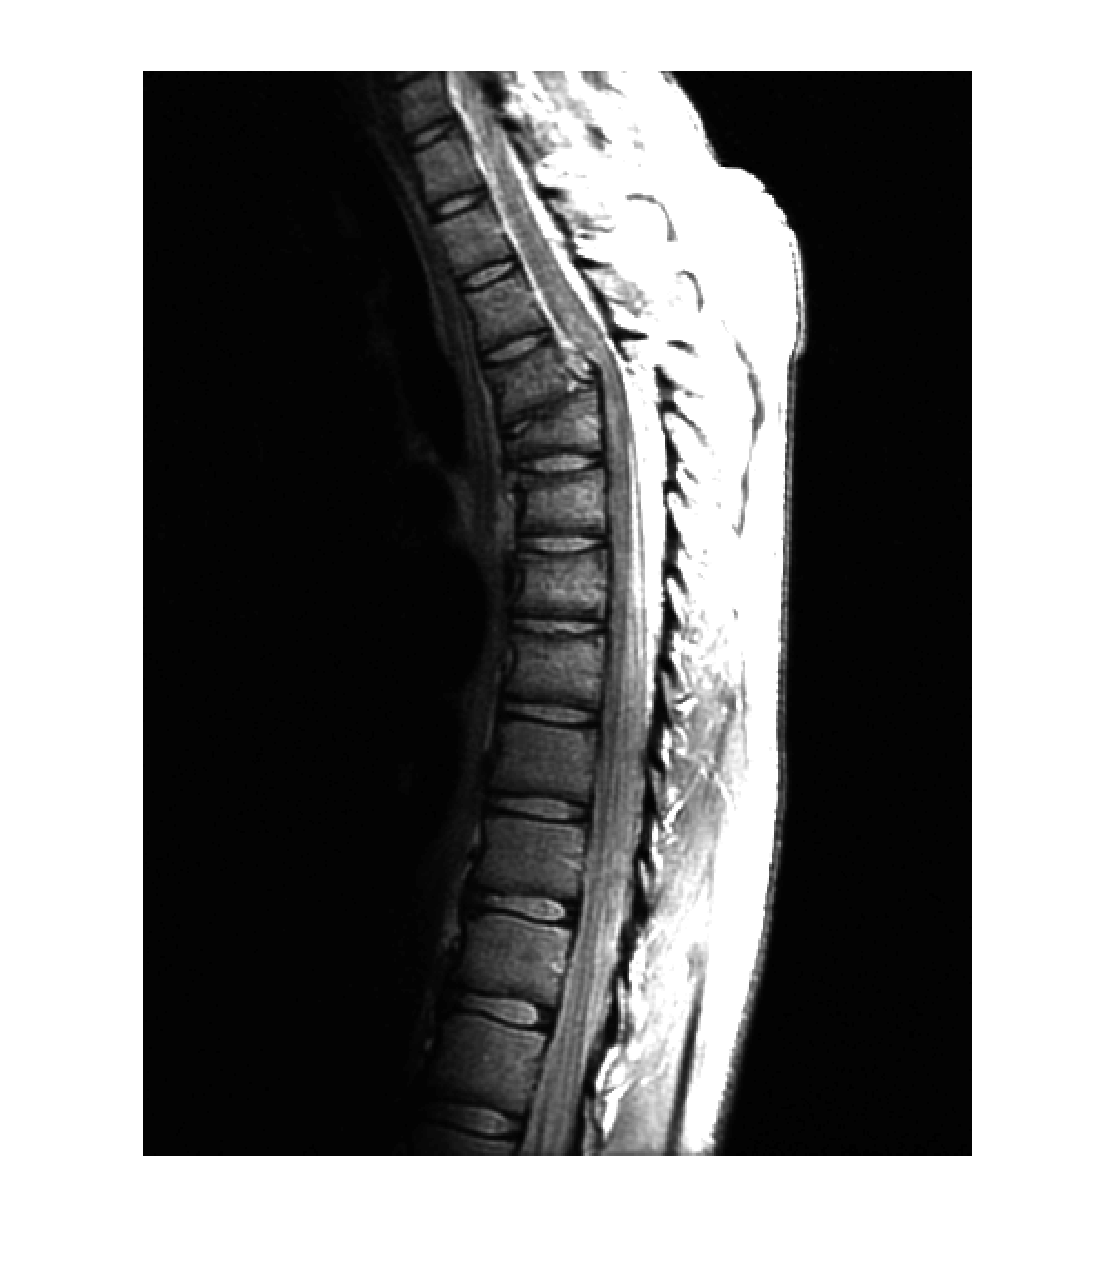
\includegraphics[width=\textwidth]{breukOokMooi.eps}
  \caption{Enhanced with \(c=3\)}
  \label{fig:withMoreEnhancement}
 \end{subfigure}
 \caption{Comparison of images of a fractured spine with and without the log transform.}
\end{figure}
\clearpage